\documentclass[a4paper]{report}
\usepackage[utf8]{inputenc}
\usepackage[affil-it]{authblk}
\usepackage{graphicx}  
\usepackage[colorlinks]{hyperref}
\usepackage{lastpage}

\usepackage[a4paper,paperwidth=9.0in,paperheight=11in]{geometry}
\title{SEC Xtractor -- Assisted Hardware Analysis Tool}

\author{Thomas Weber
  \thanks{\texttt{research@sec-consult.com}}}
\affil{SEC Consult Unternehmensberatung GmbH\footnote{\texttt{\url{https://www.sec-consult.com}}},\\ SEC Consult Vulnerability Lab,\\ Leopold-Ungar-Platz 2/3/3, 1190, Vienna\\Responsible: T. Weber, Classification: Public}

\usepackage{fancyhdr}
\usepackage{graphicx}
\pagestyle{fancy}
\fancyhf{}  
\lfoot{
\includegraphics[scale=0.25]{figure/sec-consult-logo.png}}
\rfoot{\thepage/\pageref{LastPage}}
\cfoot{\textit{SEC Consult Vulnerability Lab | Version 0.2}}
\fancyhead[R]{Classification: Public}
\fancyhead[L]{Responsible: T. Weber}
\fancyhead[C]{\today}
\renewcommand{\footrulewidth}{0.4pt}
\renewcommand{\headrulewidth}{0.4pt}
   
\fancypagestyle{plain}{
   \fancyhf{}
   \lfoot{
\includegraphics[scale=0.25]{figure/sec-consult-logo.png}}
   \rfoot{\thepage/\pageref{LastPage}}
   \cfoot{\textit{SEC Consult Vulnerability Lab | Version 0.2}}
   \fancyhead[R]{Classification: Public}
   \fancyhead[L]{Responsible: T. Weber}
   \fancyhead[C]{\today}
}

\begin{document}
\maketitle
\chapter{Overview}
This chapter gives an overview about the SEC Xtractor tool and its functionalities.
The schematics are also located here.
\section{General Description}
The SEC Xtractor Assisted Hardware Analysis Tool was originally designed as internal hardware analysis tool. 
It was used as all-in-one solution to dump NAND \/ NOR \/ SPI and I2C flash memory chips. 
Because of different voltage levels of some chips, the SEC Xtractor provides the option to adjust the voltage from 1.8V to 5.3V. 
Its program code is completely written in standard C which enables any programmer to modify the code without a lot of knowledge about hardware. 
Custom memory chips can also be added to the firmware in this way.
Beside reading flash memory chips, the SEC Xtractor has integrated JTAG-bruteforce functionality with configurable pin count. 
UART transmit pins can be found with a passive UART identifier module.
Another capability of the SEC Xtractor is the directly available FT2232H module that enables the device to use OpenOCD and two serial ports out of the box, also with configurable voltage levels.
\section{Functional Description}
This tool can be used as
\begin{itemize}
 \item memory chip reader (I2C, SPI, NAND, NOR)
 \item interface identification gadget (JTAG, UART)
 \item power supply (5V, 2.7V, 1.8-5.3V)
 \item UART to USB bridge
 \item JTAG adapter with OpenOCD
\end{itemize}

The integrated protection circuit of the level shifters (up to +/-8kV) is the reason why no external diodes were used in the schematics.
All commands that can be issued to the integrated SEC Xtractor shell can be sent by using the following UART serial port settings:
\begin{itemize}
 \item Serial Port: Two serial ports will appear when the device is attached. Take the first port \textit{(mostly ttyUSB0)}.
 \item Baudrate: 4 MBaud
 \item Configuration: No flow control, no parity bit, 8 data bit, one stop bit
\end{itemize}


\subsection{Memory Reader}
The SEC Xtractor can read I2C memory chips by using libmpsse.
SPI memory chips can be read by using the \texttt{flashrom} project.
The ATXmega128A1U is not needed for I2C and SPI.

NAND and NOR memory chips can be read by using the ATXmega128A1U microcontroller.
Both actions can be done directly over the tools command line.

\subsection{Interfaces}
A JTAG brute forcer was implemented on a modified version of JTAGenum, originally written by cyphunk aka Nathan Andrew Fain \textit{(see \url{https://deadhacker.com/2010/02/03/jtag-enumeration/})}.
To find UART interfaces, another piece of software was implemented with interrupts.
This UART scanner detects such interfaces in a passive way by just listening on the specified pins.
An RS485 transceiver can be used in a DIL socket for communicating with bus devices.
The MAX3471 transceiver is recommended for this purpose.
All other pins are protected by the internal diodes of the TXS0108E-Q1 level shifters.
They are used to shift the IO voltage levels of the ATXmega128A1U microcontroller from 1.8V to 5.3V and the voltage levels of the FT2232H microcontroller from 1.8V to 3.3V.

\subsection{Power Supply}
The board supplies 5.0V, 2.7V and adjustable voltage.
The used darlington transistors can deliver several amperes \textit{(depending on the specific model)}
It is usually enough for ~500mA devices without additional cooling of the transistors.

\textbf{Note: The power supply is not protected from short circuits!}
\subsection{UART-to-USB}
The FT2232H mini module can directly act as UART to USB converter on different voltage levels.
This can be used for connecting to a shell of a target device.

\subsection{JTAG Adapter}
The FT2232H mini module can also directly act as hardware JTAG adapter by using the OpenOCD software on different voltage levels.

\section{Board Revisions}
\subsection{Revision 1.0}
Initial revision.
Green soldermask.
\subsection{Revision 1.20}
The power supply of the FT2232H mini module and the overall system were merged. 
This resolved the power supply issues when plugging in the USB port before the power supply. 
Additional silk text was added to label the SPI pins for the FT2232H chip.
Red soldermask.
\subsection{Revision 1.31}
A boot button and two crystals (32.768kHz and 16MHz) were added to the system.
The system voltage level was changed from 3.3 volt to 2.7 volt.
Black soldermask.
\section{Schematics}
\begin{figure}[ht] 
  \centering
  {
   \setlength{\fboxsep}{0pt}
   \setlength{\fboxrule}{0pt}
   \fbox{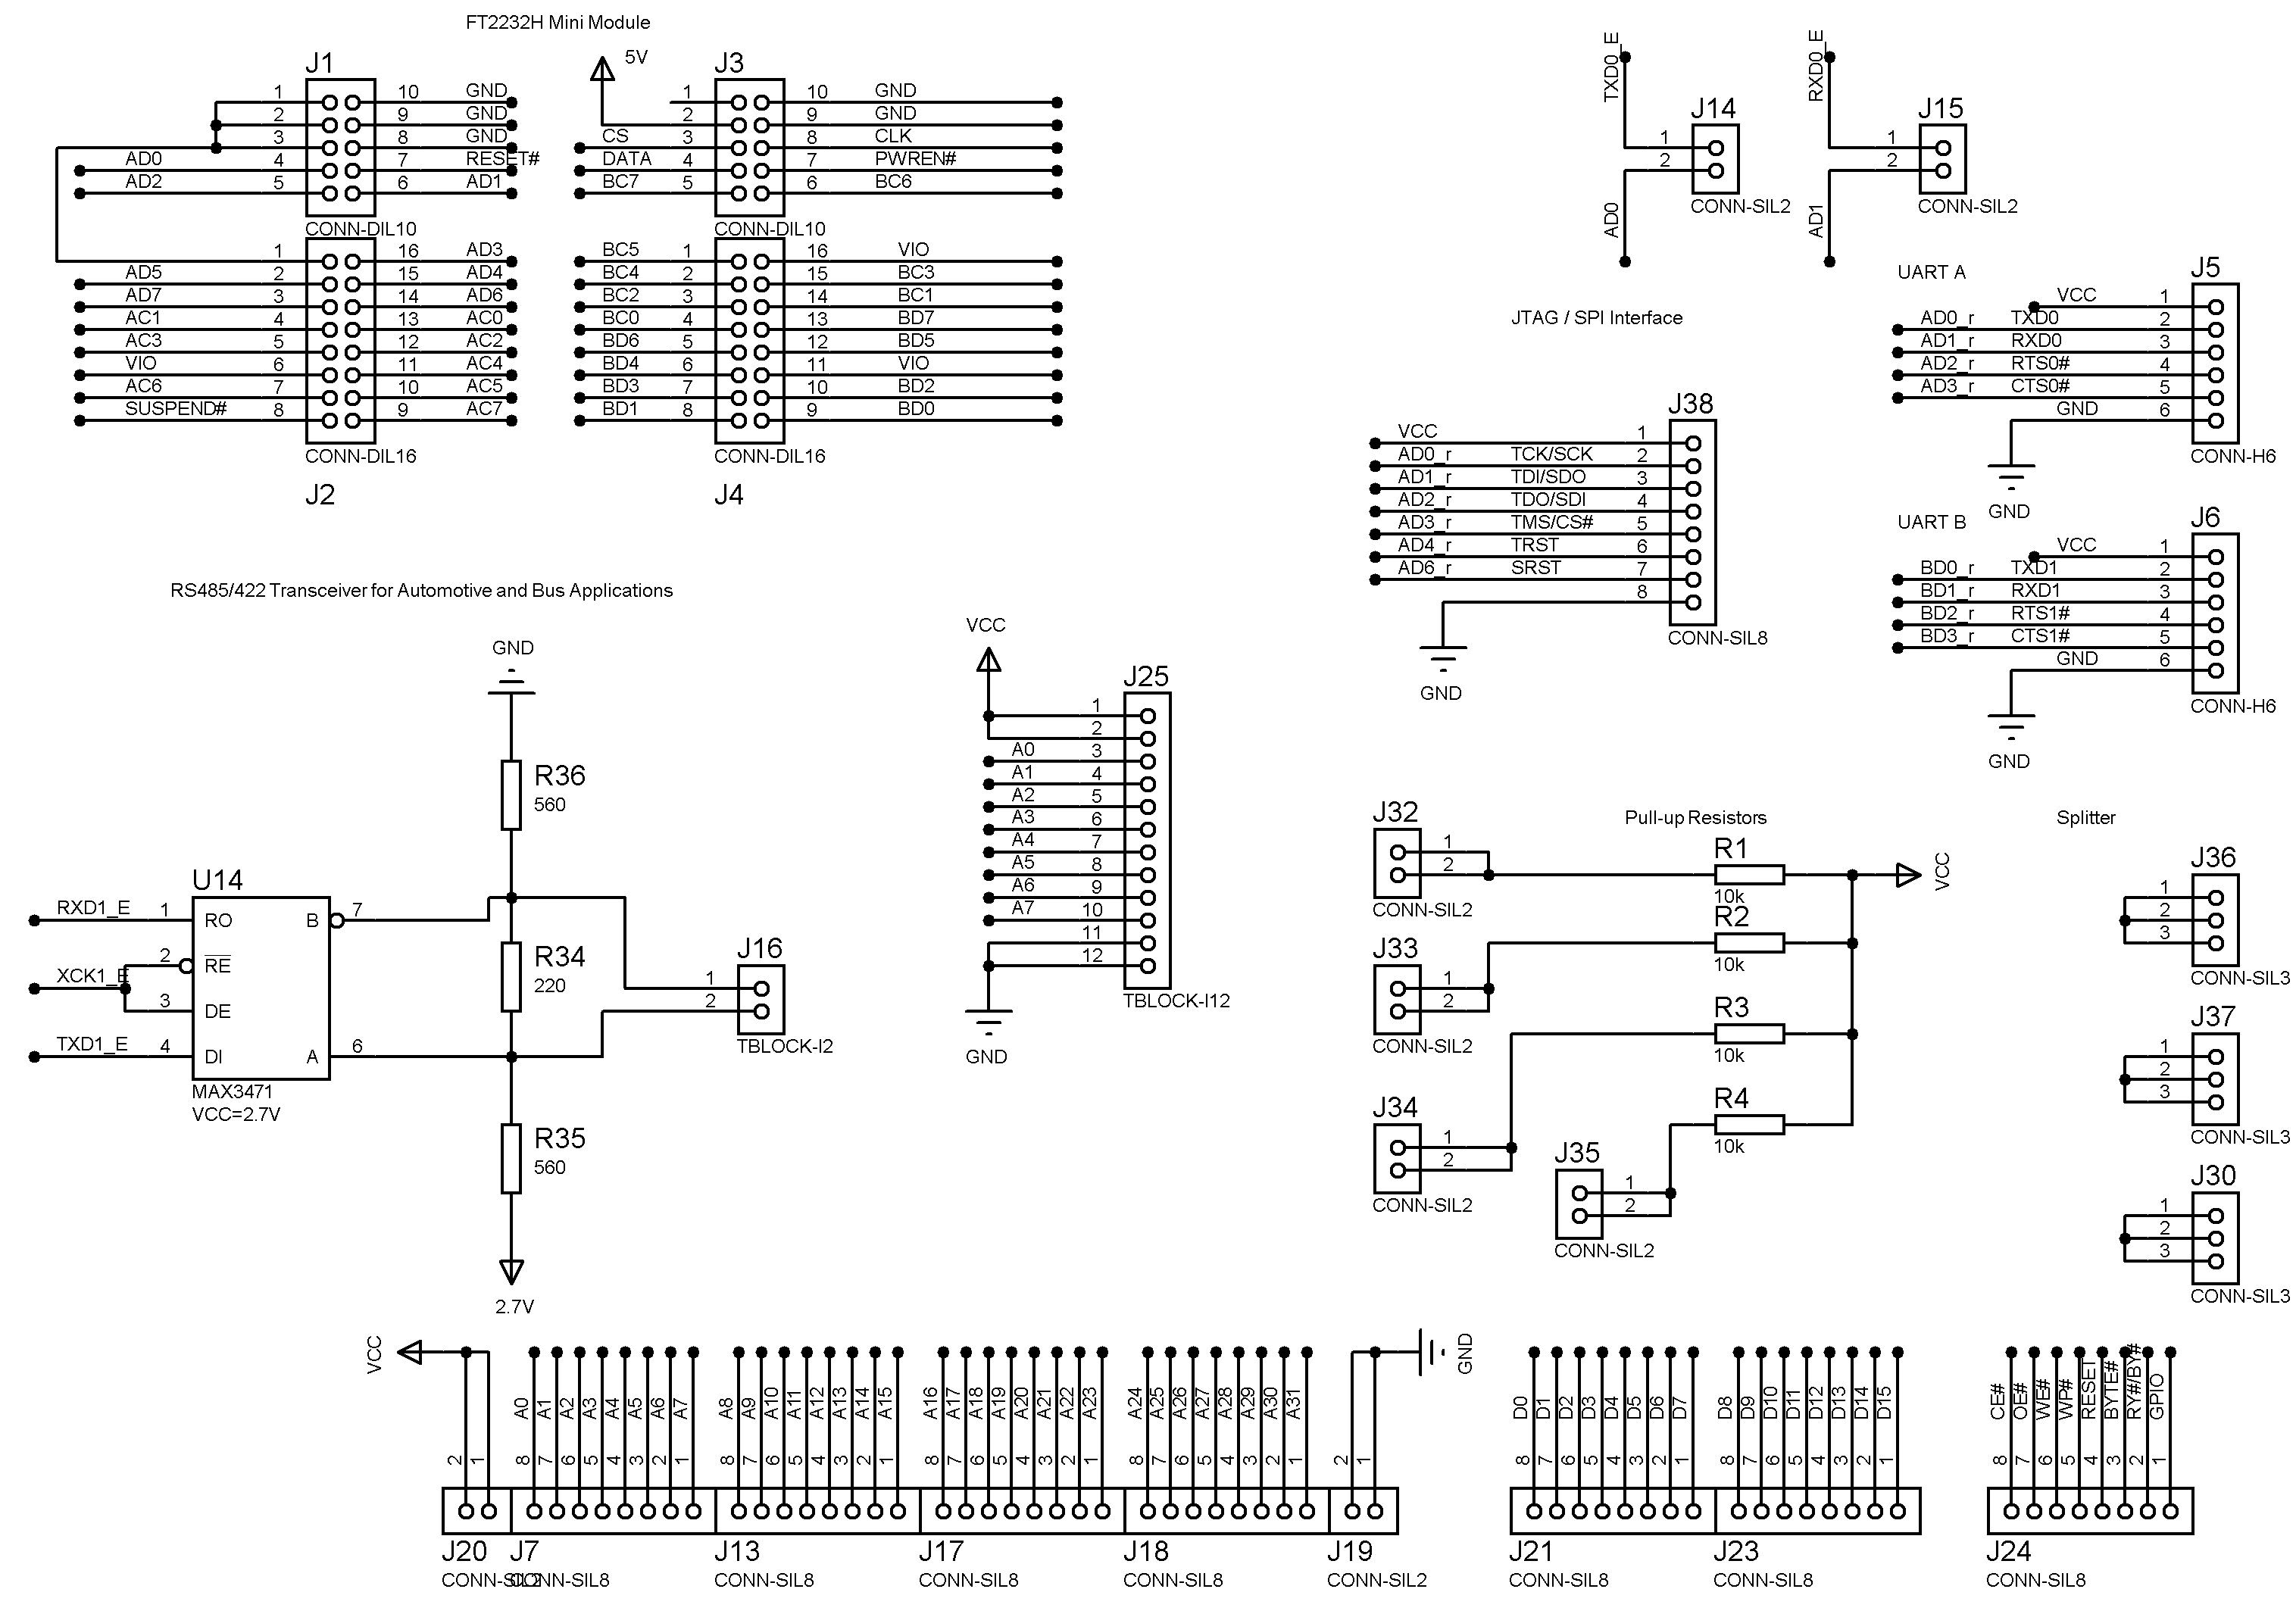
\includegraphics[width=1\textwidth]{../schematics/sec-xtractor-ft2232h.png}}
  }
  \caption{Schematics including the FT2232H mini module, the RS485 transceiver, connectors and pull-up resistors.}
  \label{fig:ft2232_schematic}
\end{figure}

\begin{figure}[ht] 
  \centering
  {
   \setlength{\fboxsep}{0pt}
   \setlength{\fboxrule}{0pt}
   \fbox{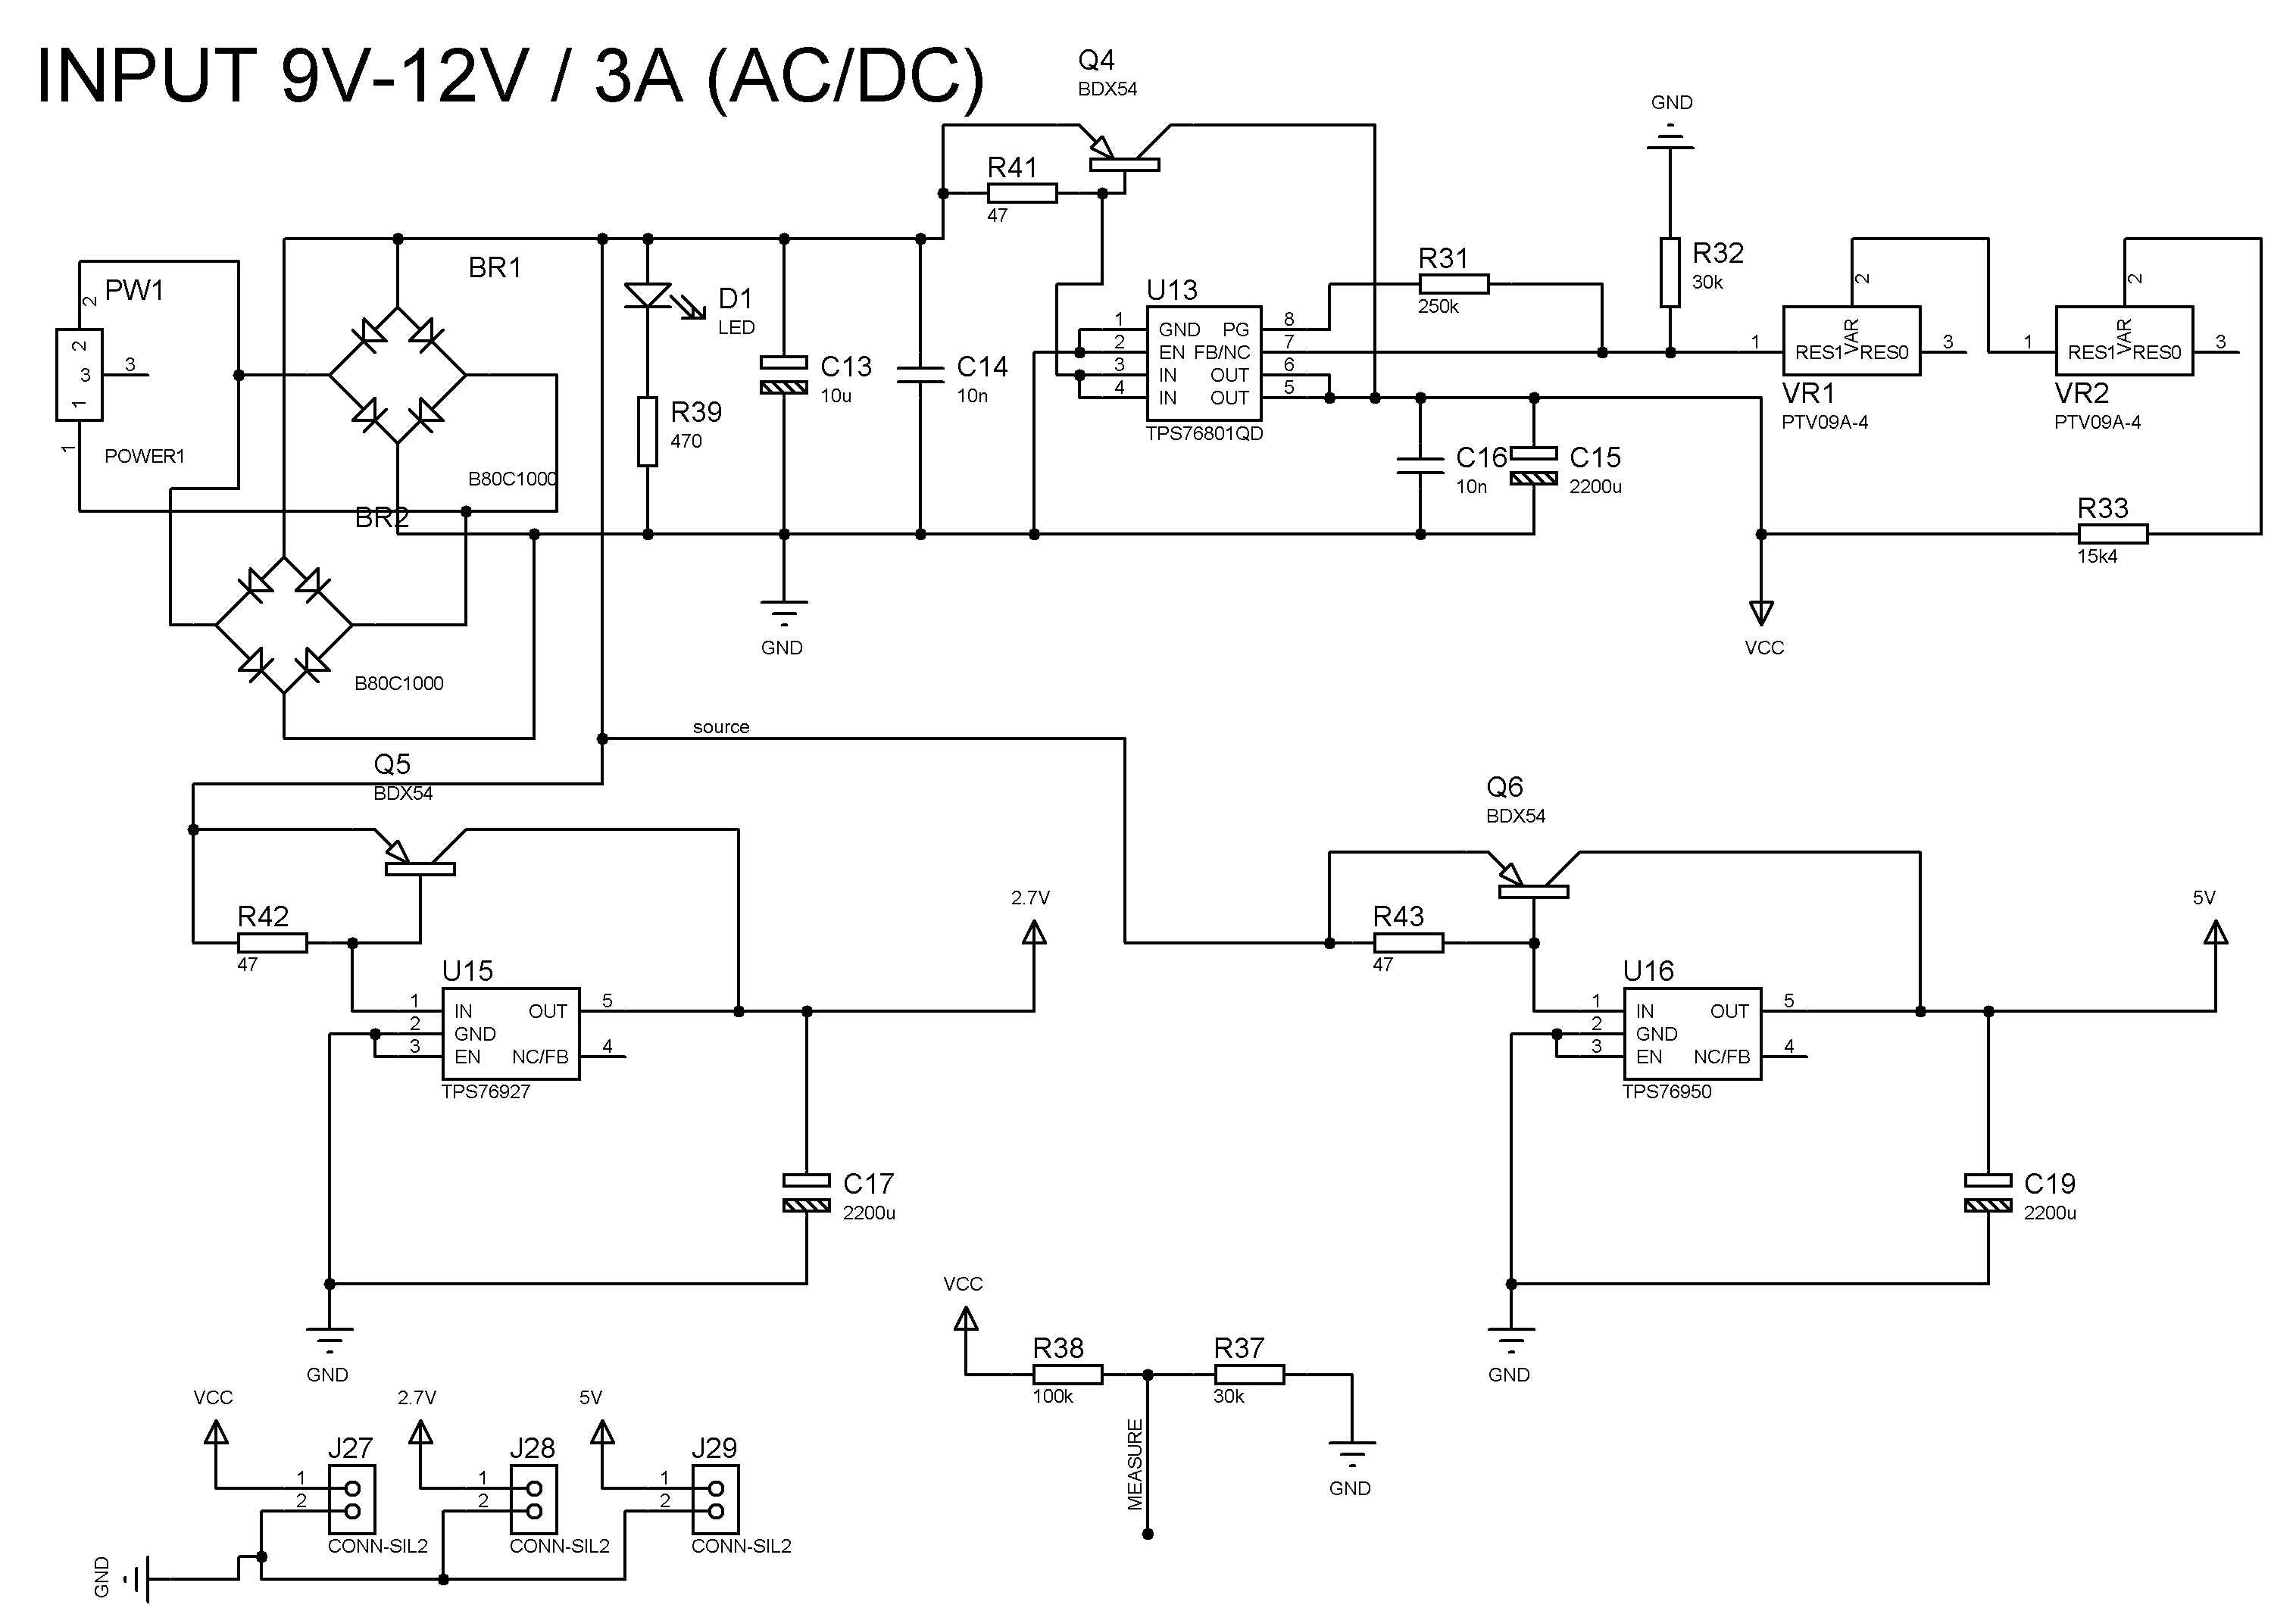
\includegraphics[width=1\textwidth]{../schematics/sec-xtractor-power.png}}
  }
  \caption{Power supply schematics of the whole board. The voltage divider for the analogue measurement is included.}
  \label{fig:power_schematic}
\end{figure}

\begin{figure}[ht] 
  \centering
  {
   \setlength{\fboxsep}{0pt}
   \setlength{\fboxrule}{0pt}
   \fbox{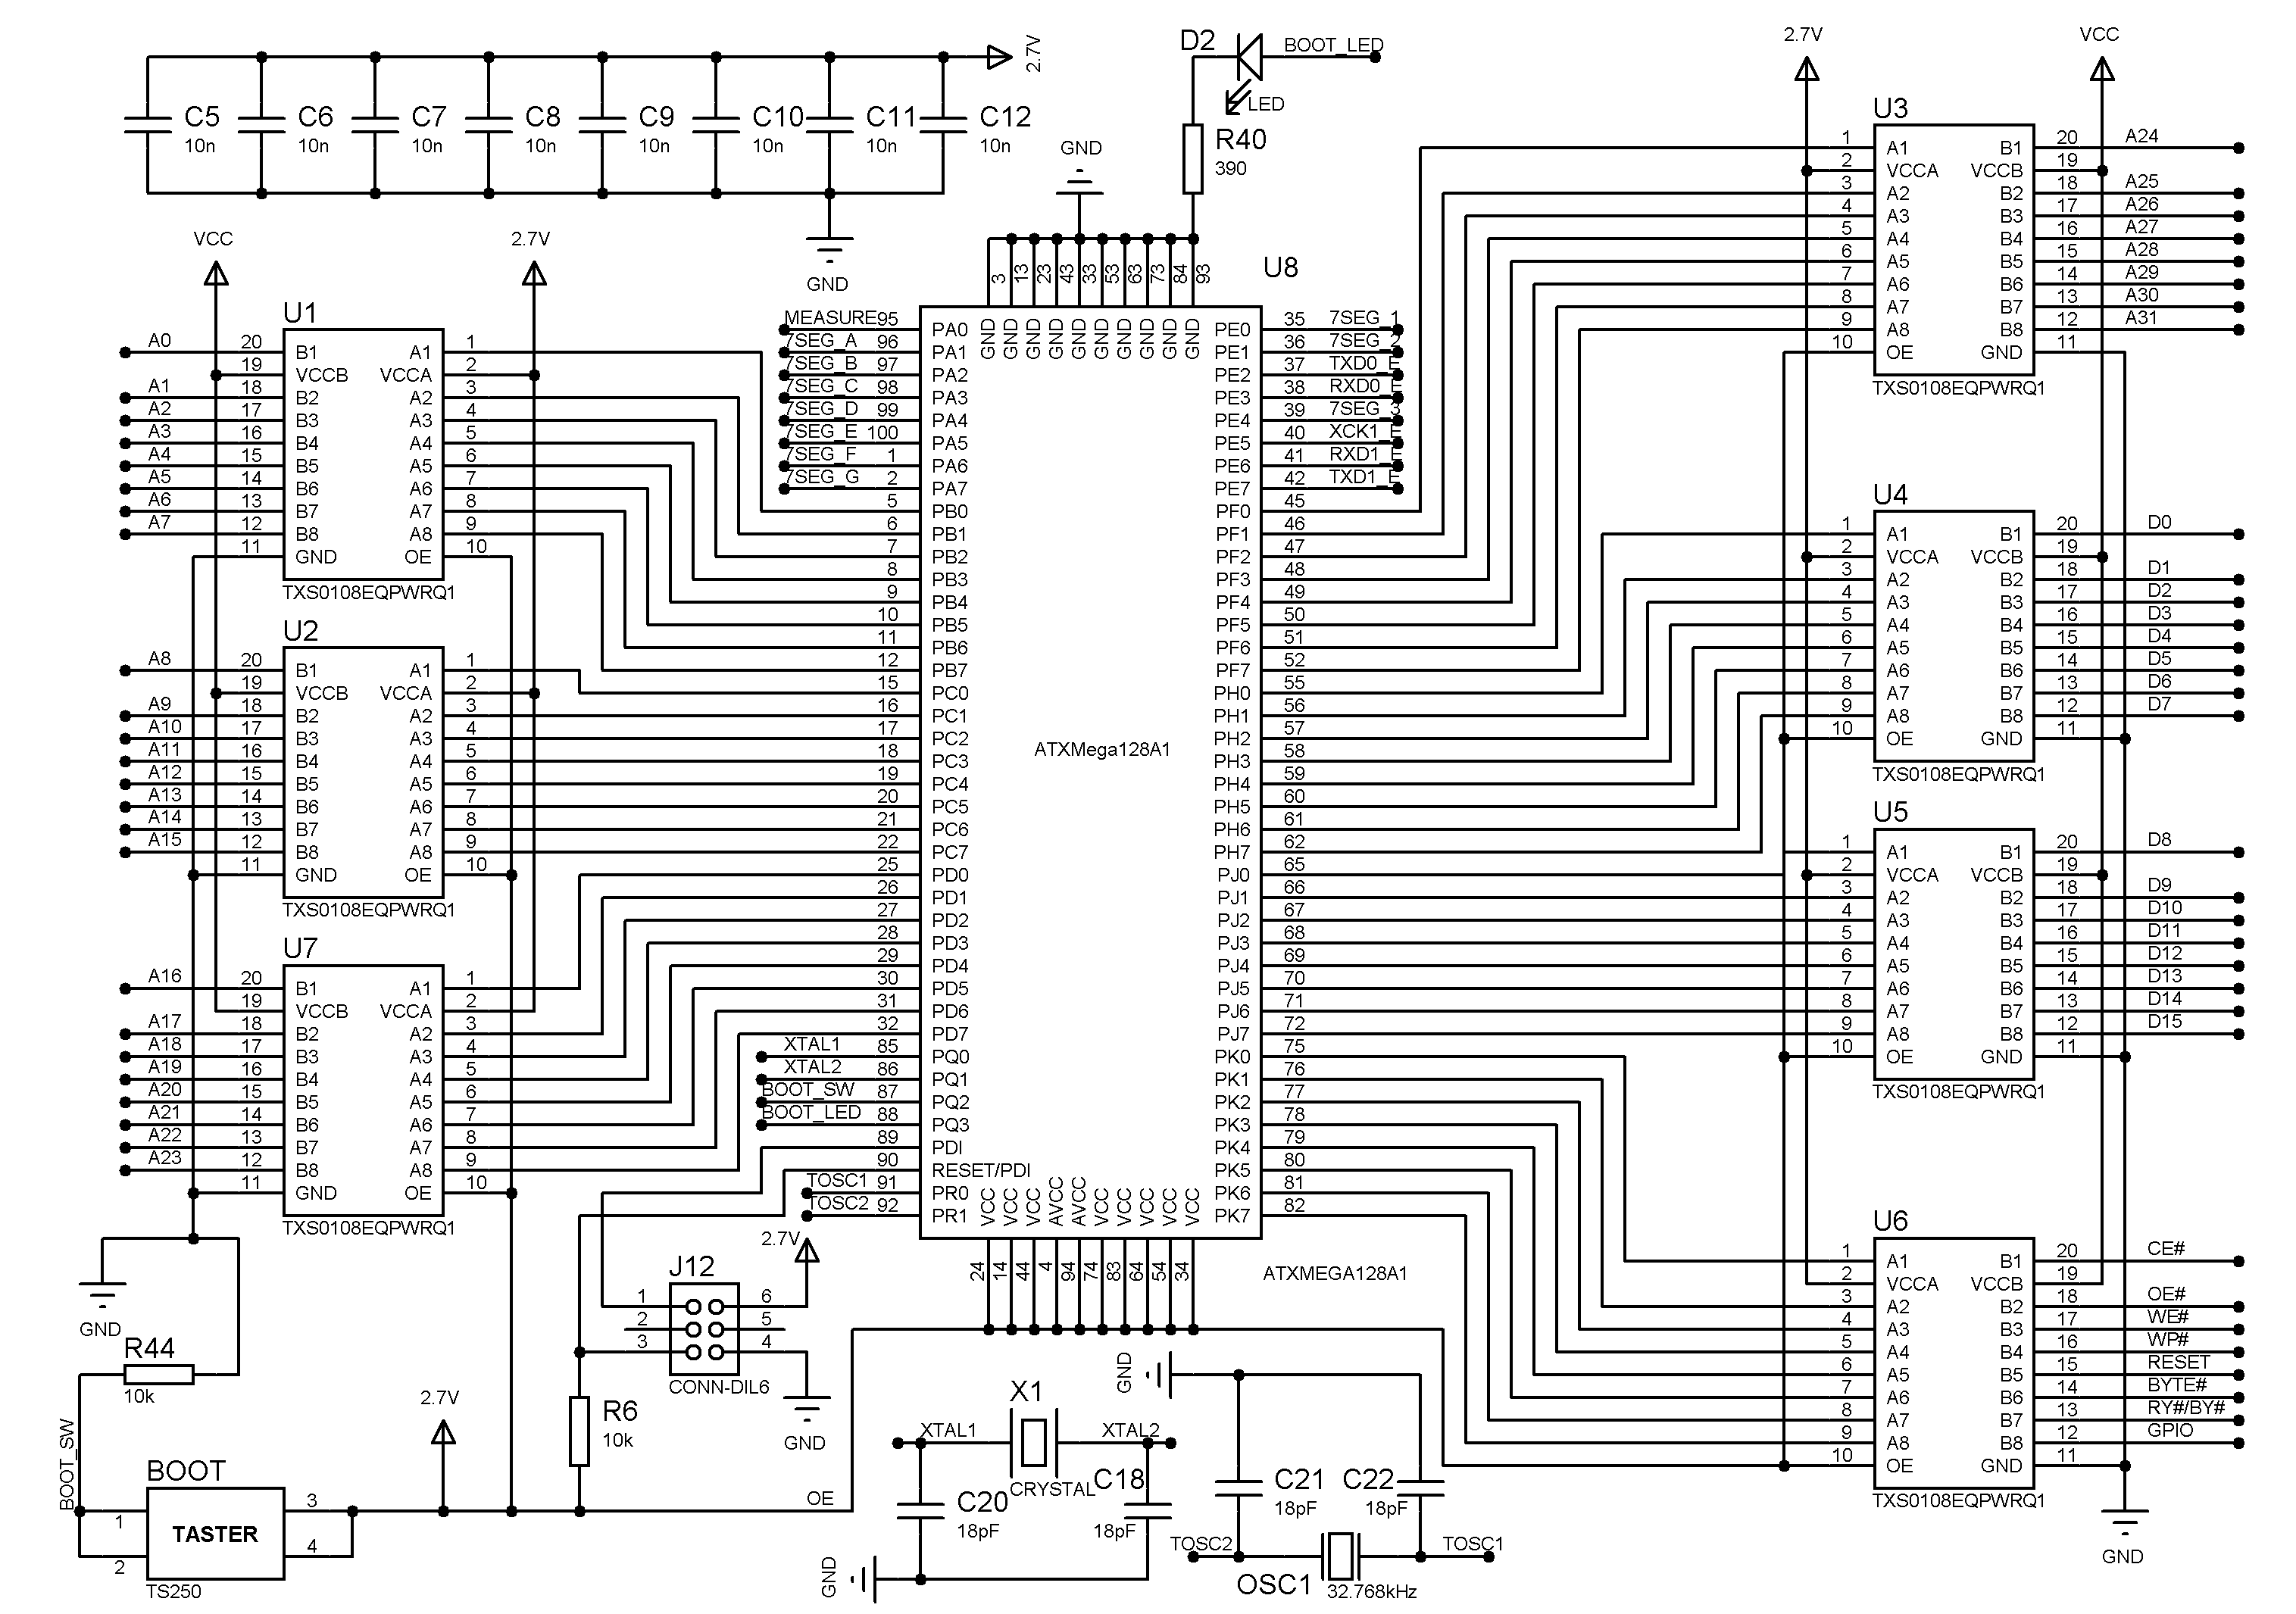
\includegraphics[width=1\textwidth]{../schematics/sec-xtractor-atxmega128a1u.png}}
  }
  \caption{This schematic sheet includes the core of the tool. The main microcontroller including peripheral components like the level shifters are depicted here.}
  \label{fig:atxmega_schematic}
\end{figure}

\begin{figure}[ht] 
  \centering
  {
   \setlength{\fboxsep}{0pt}
   \setlength{\fboxrule}{0pt}
   \fbox{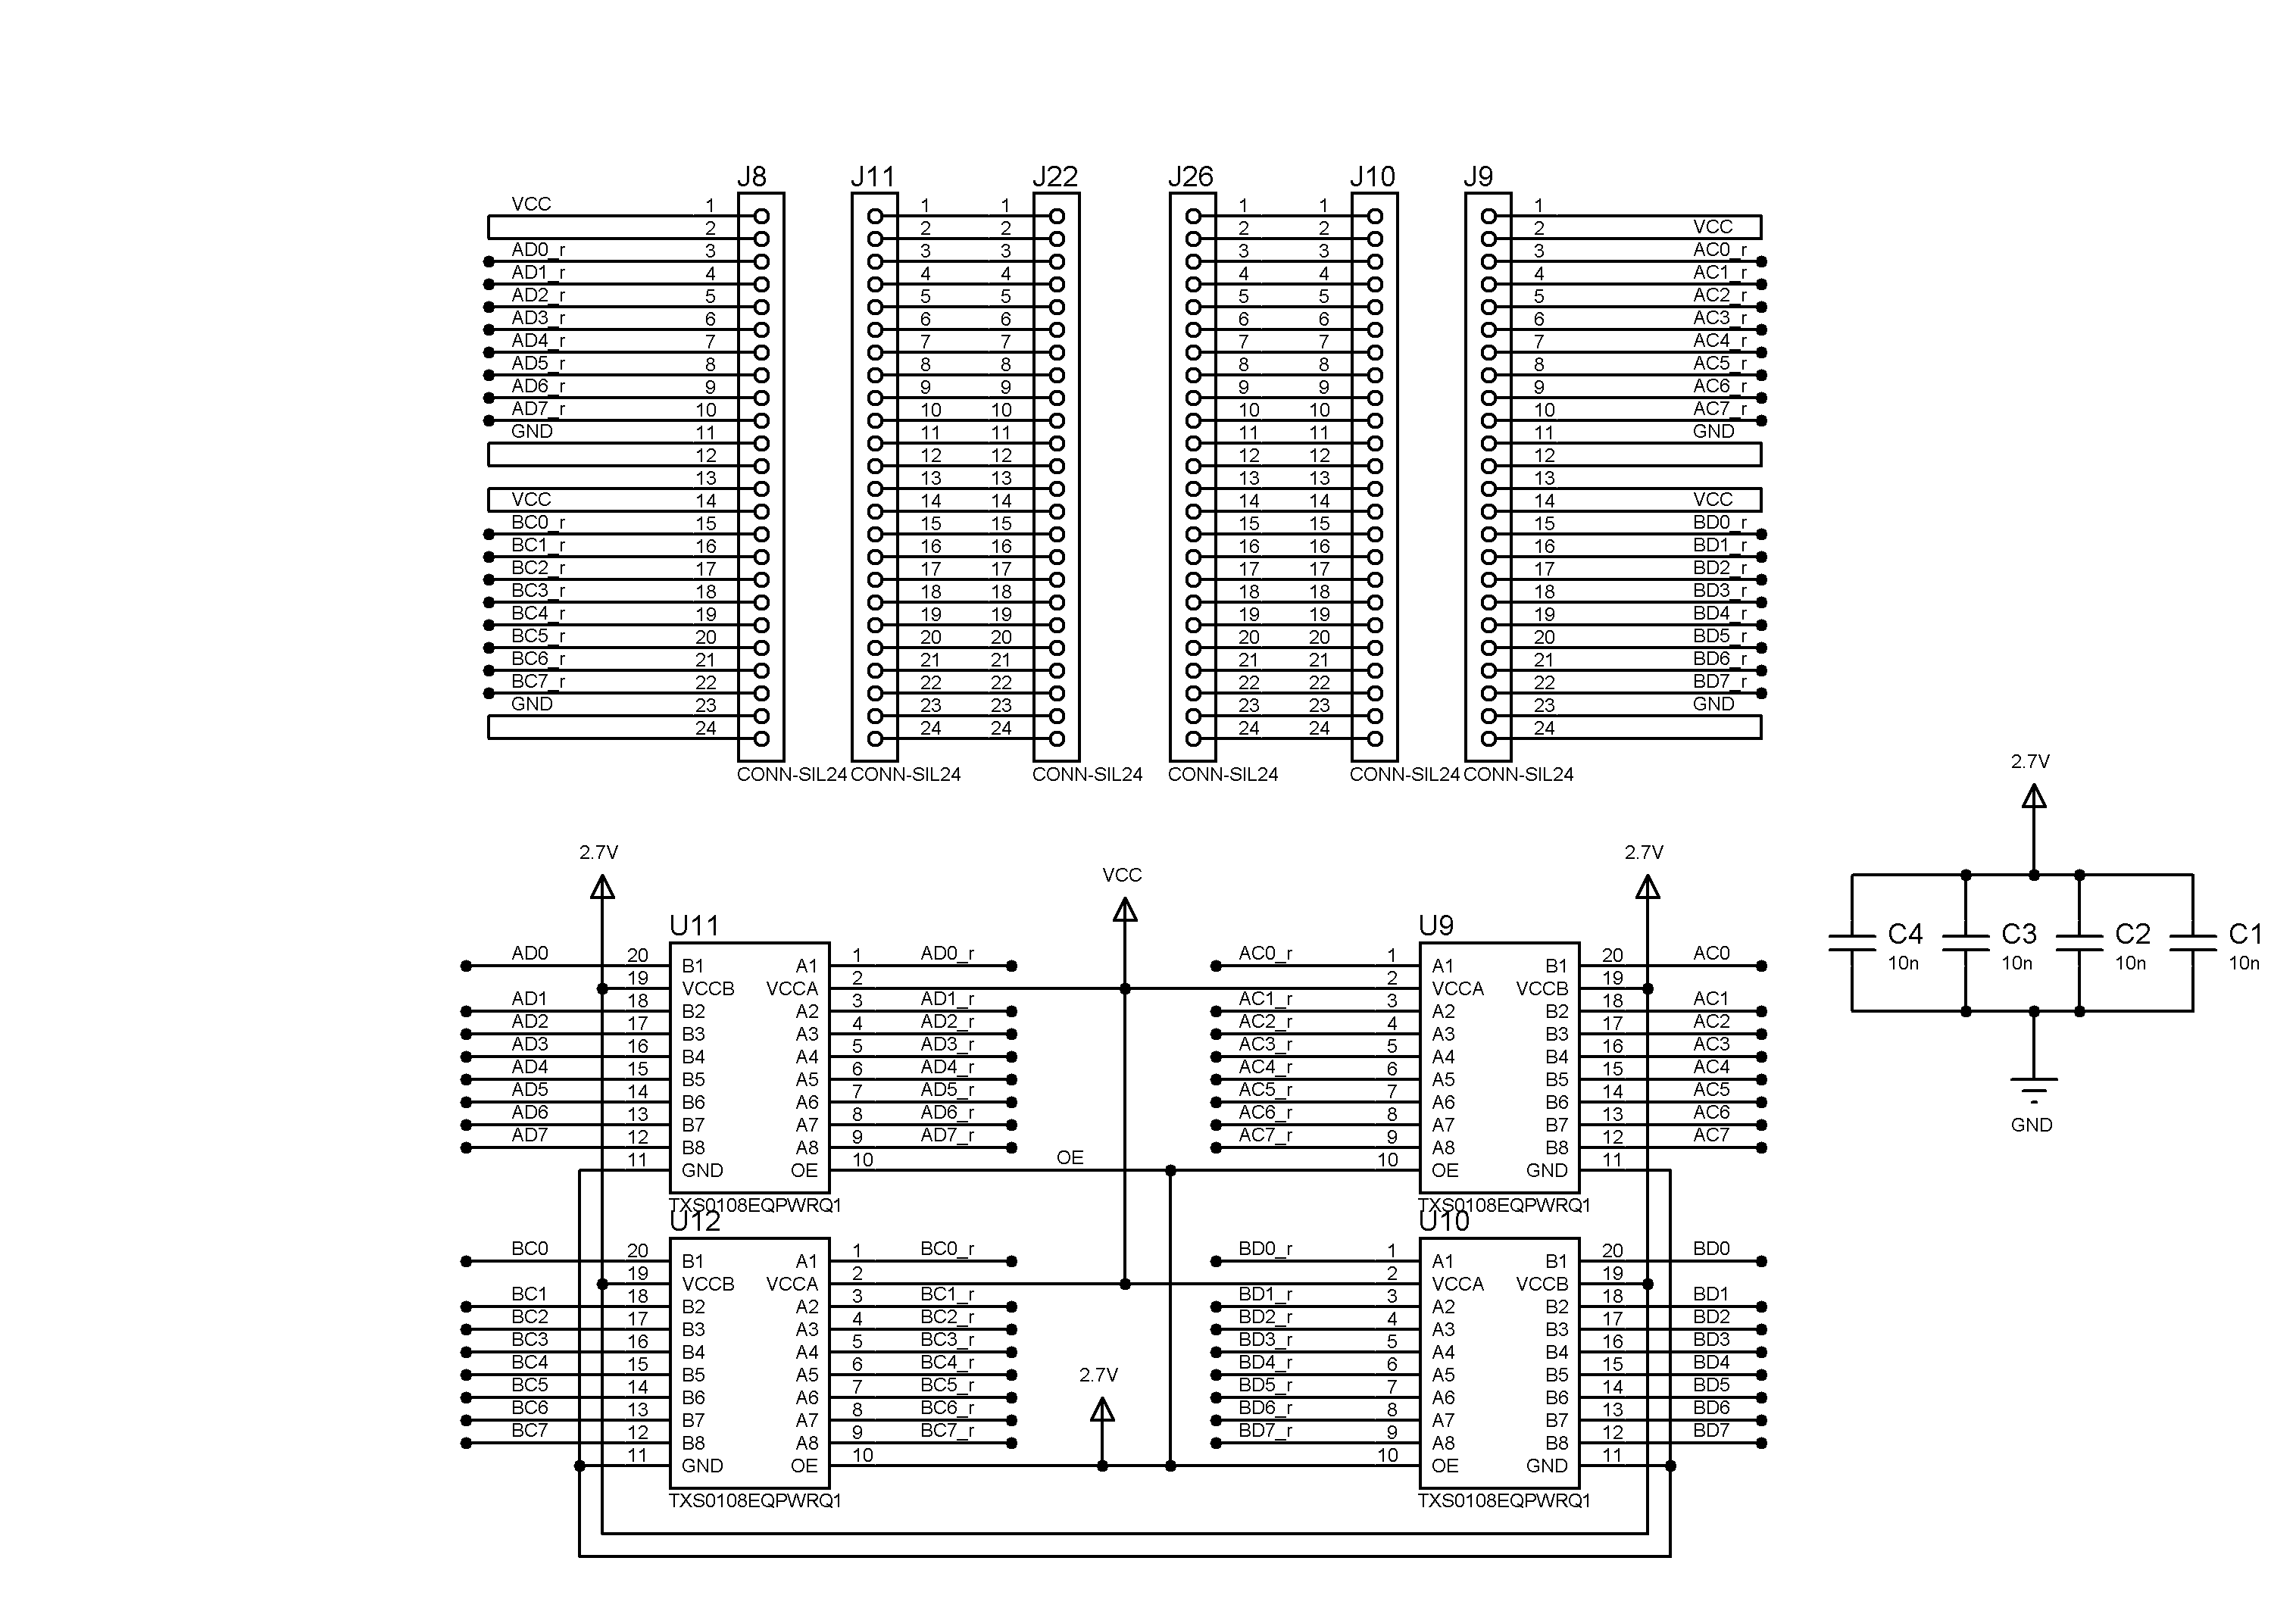
\includegraphics[width=1\textwidth]{../schematics/sec-xtractor-adapter.png}}
  }
  \caption{The ZIF adapter and level shifters are included on this schematic sheet.}
  \label{fig:adapter_schematic}
\end{figure}

\begin{figure}[ht] 
  \centering
  {
   \setlength{\fboxsep}{0pt}
   \setlength{\fboxrule}{0pt}
   \fbox{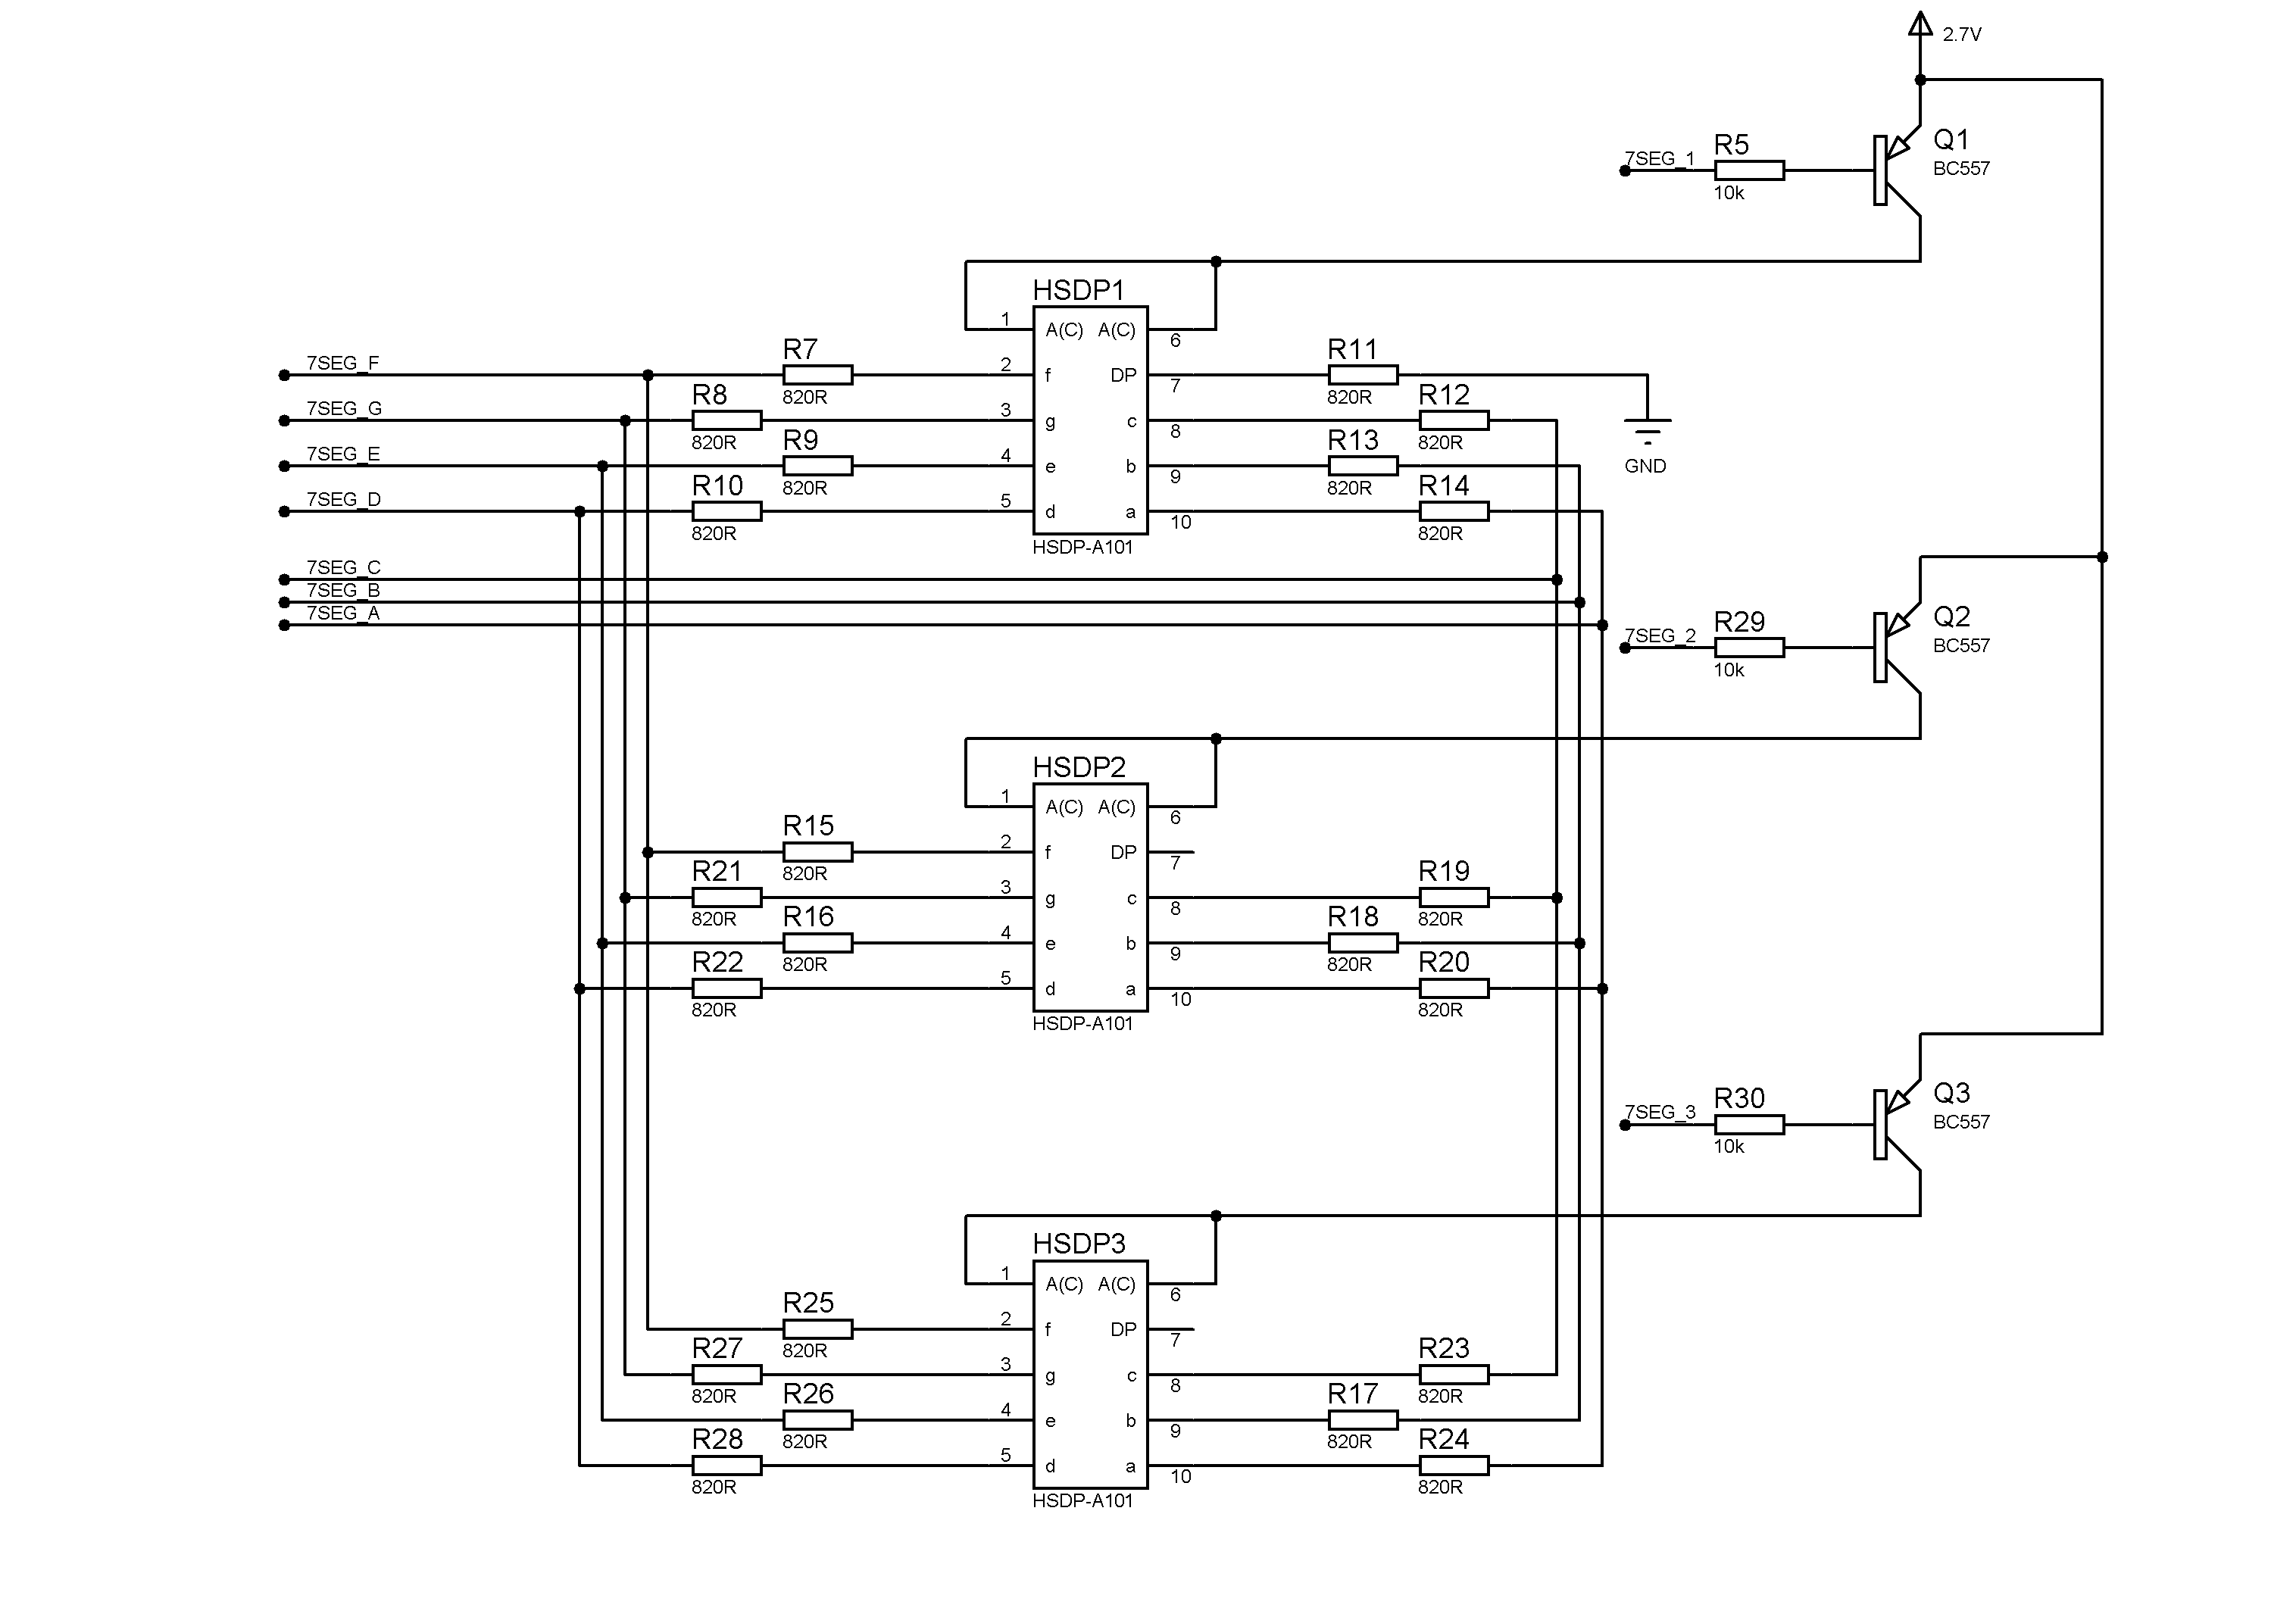
\includegraphics[width=1\textwidth]{../schematics/sec-xtractor-7segment.png}}
  }
  \caption{The seven-segment displays are included in this schematic sheet.}
  \label{fig:7seg_schematic}
\end{figure}

\chapter{Memory Reading}
The usage of the SEC Xtractor for reading memory chips is explained in this chapter.
\section{SPI}
For reading SPI flash memory chips, the SEC Xtractors ZIF socket in the center of the PCB \textit{(see Figure \ref{fig:center_socket})} is intended to be used.
\begin{figure}[ht] 
  \centering
  {
   \setlength{\fboxsep}{0pt}
   \setlength{\fboxrule}{0.5pt}
   \fbox{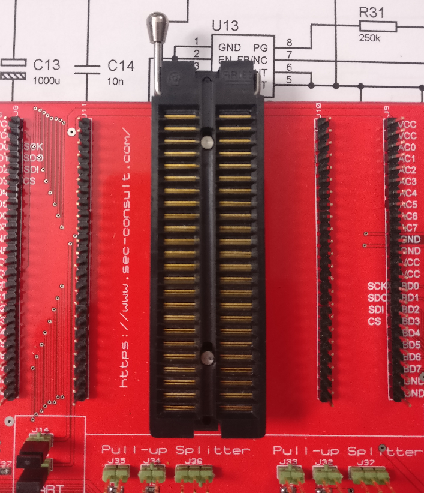
\includegraphics[width=0.35\textwidth]{../photos/zif_socket.png}}
  }
  \caption{ZIF socket in the center of the SEC Xtractor tool.}
  \label{fig:center_socket}
\end{figure}
By attaching an appropriate DIL adapter to the socket \textit{(see Figure \ref{fig:attached_adapter})}, a broad range of SMD chips can be read.
\begin{figure}[ht] 
  \centering
  {
   \setlength{\fboxsep}{0pt}
   \setlength{\fboxrule}{0.5pt}
   \fbox{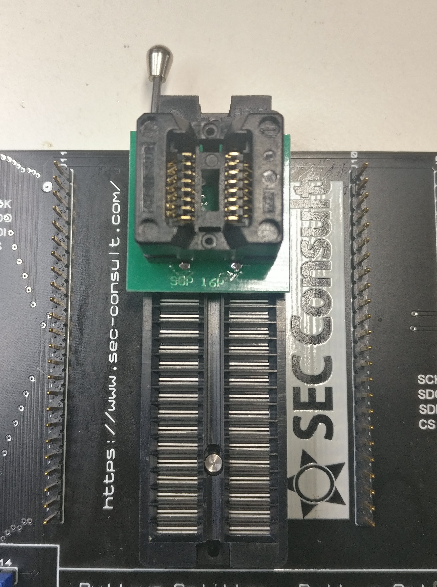
\includegraphics[width=0.35\textwidth]{../photos/dil_adapter.png}}
  }
  \caption{Mounted DIL adapter for SOP16 packages.}
  \label{fig:attached_adapter}
\end{figure}
It is important to open the UART bridge of the ATXmega128A1U when reading from channel A of the FT2232H chip as both ICs would be attached at the same time in this case.
This can result in interferences which disrupts the communication.
Channel B can be used without any jumper changes.
\begin{figure}[ht] 
  \centering
  {
   \setlength{\fboxsep}{0pt}
   \setlength{\fboxrule}{0.5pt}
   \fbox{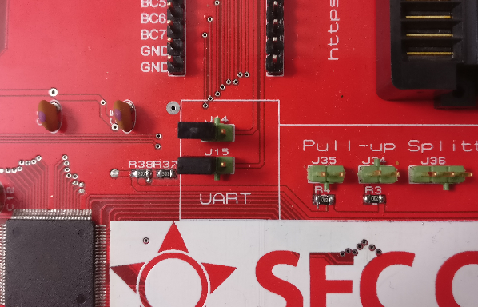
\includegraphics[width=0.35\textwidth]{../photos/open_uart_bridge.png}}
  }
  \caption{UART jumper bridge to the ATXmega128A1U.}
  \label{fig:uart_jumper}
\end{figure}
The project \texttt{flashrom} \textit{(see https://flashrom.org/)} can be used to dump SPI memory chips.
Because of the propagation delay, that comes form the level shifters, a clock divisor for the read and write command should be used.
A normal read operation can be started by issuing the following command:

\texttt{flashrom -p ft2232\_spi:type=2232H,port=A,divisor=10 -r dump.bin}

To connect a SPI memory chip for reading purpose, the circuitry depicted in Figure \ref{fig:SPI_circuit} can be used.
\begin{figure}[ht] 
  \centering
  {
   \setlength{\fboxsep}{0pt}
   \setlength{\fboxrule}{0.5pt}
   \fbox{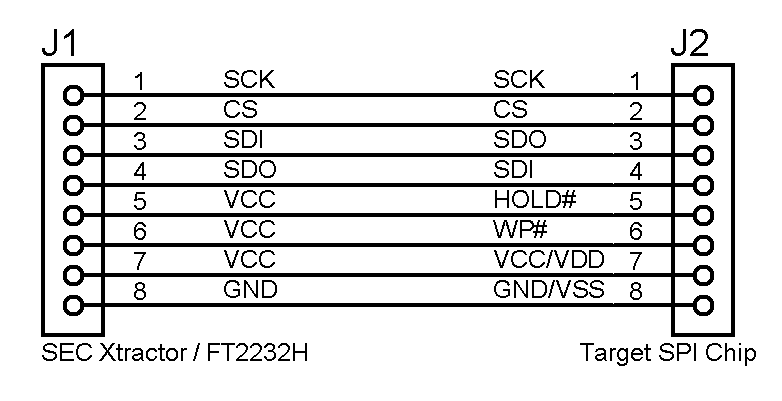
\includegraphics[width=0.35\textwidth]{../schematics/spi_target.png}}
  }
  \caption{SPI flash memory connection circuit.}
  \label{fig:SPI_circuit}
\end{figure}
To create this circuit on the SEC Xtractor board, connection wires like on prototyping boards can be used.
\section{I2C}
For reading I2C flash memory chips, the SEC Xtractors ZIF socket in the center of the PCB \textit{(see \ref{fig:center_socket})} is intended to be used \textit{(like for SPI)}.
The implication for the UART bridge, described in the previous section, is the same.
Therefore, it should be opened.
To read I2C memory chips, \texttt{libmpsse} can be used.
Repositories are available under the following links: 

\textit{\url{https://www.ftdichip.com/Support/SoftwareExamples/MPSSE/LibMPSSE-I2C.htm}}

\textit{\url{https://github.com/devttys0/libmpsse}}

To connect an I2C memory for reading purpose, the circuitry depicted in Figure \ref{fig:i2c_circuit} can be used.
\begin{figure}[ht] 
  \centering
  {
   \setlength{\fboxsep}{0pt}
   \setlength{\fboxrule}{0.5pt}
   \fbox{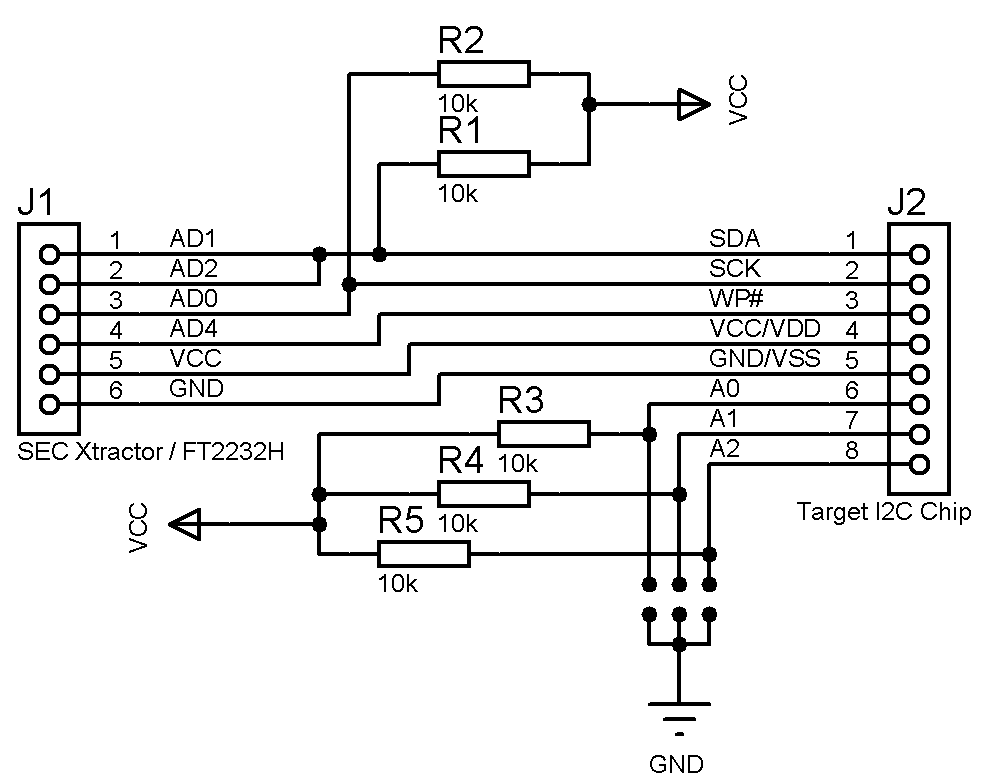
\includegraphics[width=0.40\textwidth]{../schematics/i2c_target.png}}
  }
  \caption{I2C flash memory connection circuit.}
  \label{fig:i2c_circuit}
\end{figure}
The depicted circuit is more complex than the SPI circuit in the previous section.
It can be created with prototyping wires too, but this time the \texttt{``pull-up splitter''} resistors and connectors on the SEC Xtractor \textit{(see Figure \ref{fig:center_socket})} must be used.
The address pins A0-A2 can be configured to fit to the corresponding application that reads the memory content.
\section{NOR}
For reading NOR flash memory chips, the SEC Xtractor's socket adapter can be used. 
It is located on the edge where the ATXmega128A1U resides \textit{(see Figure \ref{fig:nor_nand_socket})}.
The pins marked with \texttt{A0-A31} are the address pins, the pins marked with \texttt{D0-D15} are the data pins.
The remaining pins like \texttt{CE\#} or \texttt{RESET} are control pins.
Therefore, a maximum of 32 address bits and 16 data bits can be handled which is equal to a maximum of 68719476736 bits or 8589934592 bytes memory size.
\begin{figure}[ht] 
  \centering
  {
   \setlength{\fboxsep}{0pt}
   \setlength{\fboxrule}{0.5pt}
   \fbox{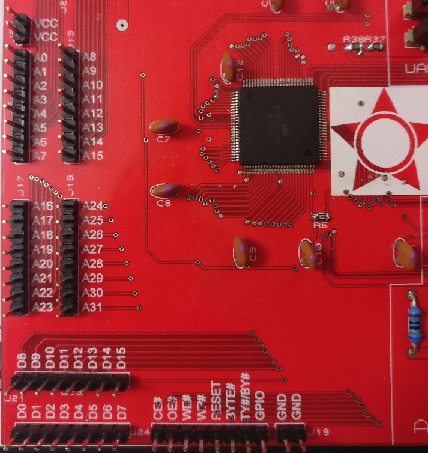
\includegraphics[width=0.40\textwidth]{../photos/nand_nor_adapter_socket.png}}
  }
  \caption{Pins that can be used for NOR and NAND flash memory chips.}
  \label{fig:nor_nand_socket}
\end{figure}

For this purpose, the UART bridge on the board must be closed \textit{(see Figure \ref{fig:uart_jumper})}.
The command ``dump nor'' can be used to read out NOR flash memory content. 
The resulting output must be converted with ``xxd -r'' to a readable binary file.

The additional adapter for NOR flash memory chips is depicted in Figure \ref{fig:nor_pcb}.
\begin{figure}[ht] 
  \centering
  {
   \setlength{\fboxsep}{0pt}
   \setlength{\fboxrule}{0.5pt}
   \fbox{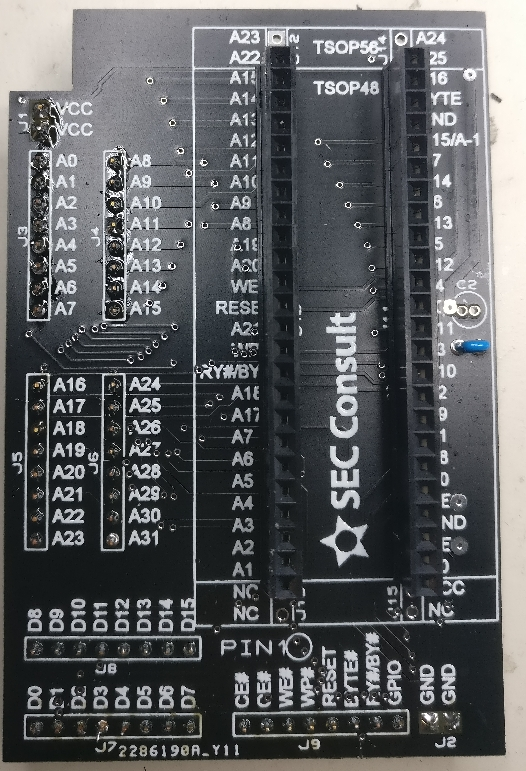
\includegraphics[width=0.40\textwidth]{../photos/nor_adapter.png}}
  }
  \caption{Adapter PCB to use NOR flash memory chips with a DIL socket.}
  \label{fig:nor_pcb}
\end{figure}
An example how it can be mounted is depicted on Figure \ref{fig:mounted_nor}.
\begin{figure}[ht] 
  \centering
  {
   \setlength{\fboxsep}{0pt}
   \setlength{\fboxrule}{0.5pt}
   \fbox{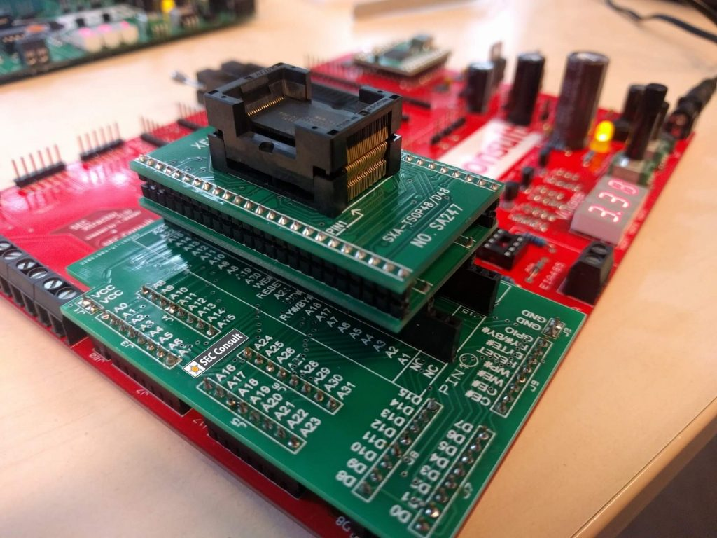
\includegraphics[width=0.40\textwidth]{../photos/mounted_nor_flash.png}}
  }
  \caption{Mounted NOR flash memory adapter with ZIF socket.}
  \label{fig:mounted_nor}
\end{figure}
A standard Xeltex SA247 TSOP-48 adapter was mounted directly with the corresponding memory chip.

\section{NAND}
Reading NAND flash memory chips can be done with the same hardware interface \textit{(see Figure \ref{fig:mounted_nand})} in a similar way like NOR flash memory chips, explained in the previous section.
A significant difference is the fact that the NAND interface, called ONFI, sends address and data commands on the same wires.
The pins marked with \texttt{D0-D15} are used for this purpose while the control pins on the SEC Xtractor are the same.
Reading out NAND memory chips can be done with the command ``dump nand'' \textit{(see Figure \ref{fig:terminal_nand})}. 
The resulting output must be converted with ``xxd -r'' to a readable binary file, as mentioned for NOR in the last section.
\begin{figure}[ht] 
  \centering
  {
   \setlength{\fboxsep}{0pt}
   \setlength{\fboxrule}{0.5pt}
   \fbox{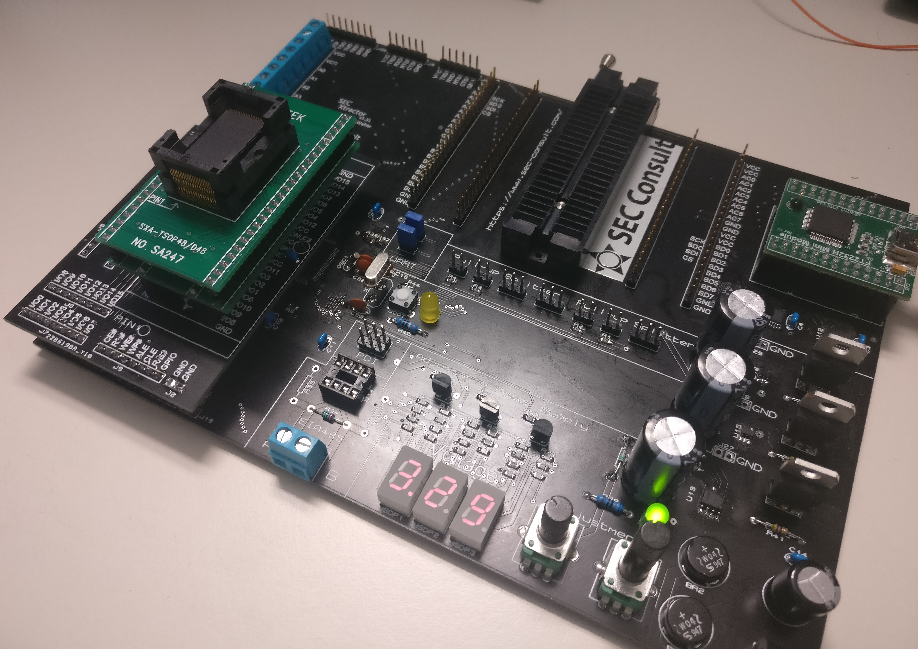
\includegraphics[width=0.40\textwidth]{../photos/mounted_nand.png}}
  }
  \caption{Mounted NAND adapter on the SEC Xtractor.}
  \label{fig:mounted_nand}
\end{figure}
\begin{figure}[ht] 
  \centering
  {
   \setlength{\fboxsep}{0pt}
   \setlength{\fboxrule}{0.5pt}
   \fbox{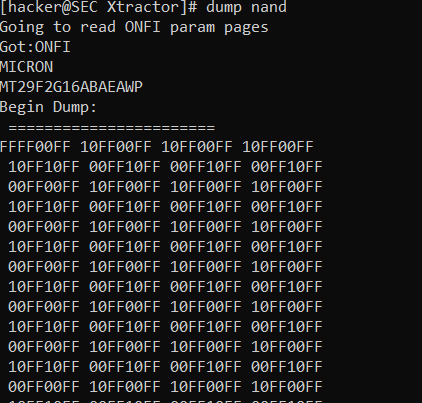
\includegraphics[width=0.40\textwidth]{../photos/terminal.png}}
  }
  \caption{Terminal output during read operation.}
  \label{fig:terminal_nand}
\end{figure}
\chapter{Interface Identification}
The interface identification functionalities are covered in this chapter.
A general command that can be issued on the SEC Xtractor shell for configuring the pin count is ``pinlen set''.
Setting the pin count of 16 for example will activate the pins ``A0''-``A15''.
\section{JTAG Identification}
JTAG can be found by connecting the corresponding wires to the target device and type ``pattern scan'', like implemented in JTAGenum.
\section{UART Detection}
The passive UART scan can be started by issuing the command ``uart scanner'' in the console. It counts the pin changes and let you determine where UART TX pins may be located.
\chapter{Firmware Development}
\section{Program the Device}
There are two ways to program the SEC Xtractor's flash memory.
The first is the classic way via the PDI port, the second way is the bootloader over the serial port.

The PDI socket can be used with all fitting AVR programmers. The AVRISPMKII is set as programmer in the Makefile. This must be changed when another programmer is used.

The bootloader mode can be initialized when the button ``BOOT'' is pressed on the PCB down during power-up and programming.
The bootloader can handle input from avrdude when the programmer ``avr911'' is set in the Makefile. 
This is the case when the command ``make flash-main-serial'' is issued. 
\end{document}          
